\section{TSP z wykorzystaniem algorytmu memetycznego}

Badania wykonano w identyczny sposób i z identycznymi parametrami, co w przypadku punktu TSP, jedyną modyfikację zaś wprowadzono ustawiając w funkcji GA

\textit{optim = T}

Przekłada się to na polecenie wykorzystania algorytmu genetycznego hybrydowego (memetycznego) przy optymalizacji.

\subsection{Wyniki}

\begin{figure}[H]
    \centering
    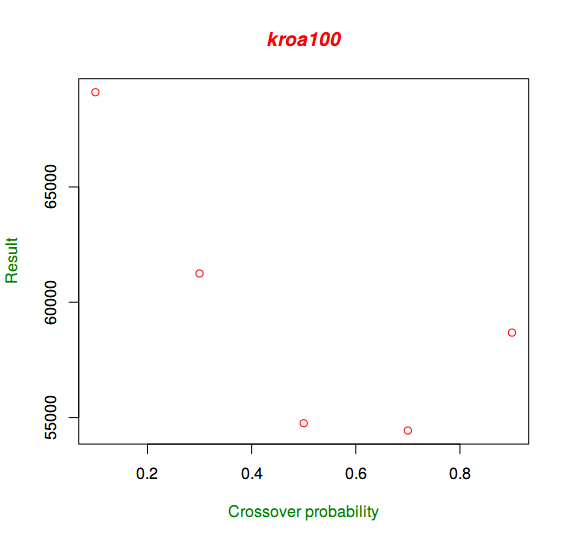
\includegraphics[scale=0.6]{tspMemetic/kroA100_pcross_result.png}
    \caption{Rezultat optymalizacji dla różnych wartościach prawdopodobieństwa krzyżowania}
\end{figure}

\begin{figure}[H]
    \centering
    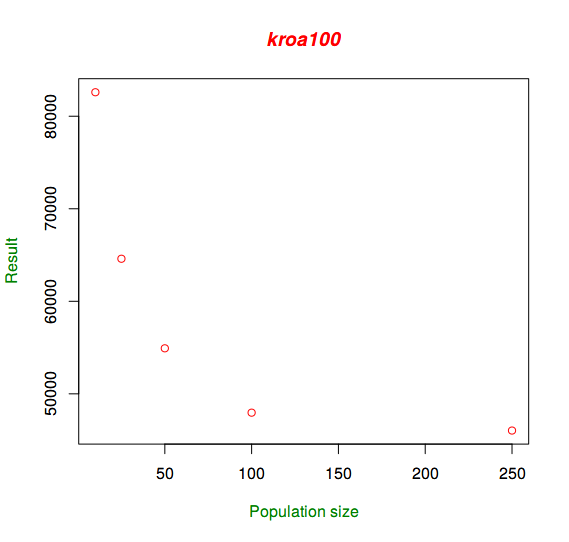
\includegraphics[scale=0.6]{tspMemetic/kroA100_popSize_result.png}
    \caption{Rezultat optymalizacji dla różnych wielkości populacji}
\end{figure}


\subsection{Wnioski}

Wyniki dla algorytmu memetycznego są identyczne z wynikami powstałymi bez jego wykorzystania.
